\documentclass[UTF8]{ctexart}
\usepackage{amsmath}
\usepackage{bm}
\usepackage{geometry}
\usepackage{graphicx}
\usepackage{amssymb} 
\usepackage{amsmath}
\usepackage{fancyhdr}
\usepackage{pythonhighlight}
\usepackage{enumerate}

\lstset{frame=tb,
  language=Python,
  aboveskip=3mm,
  belowskip=3mm,
  showstringspaces=false,
  columns=flexible,
  basicstyle={\middle\ttfamily},
  numbers=left,%设置行号位置none不显示行号
  %numberstyle=\tiny\courier, %设置行号大小  
  numberstyle=\tiny\color{gray},
  keywordstyle=\color{blue},
  commentstyle=\color{green},
  stringstyle=\color{mauve},
  breaklines=true,
  breakatwhitespace=true,
  escapeinside=``,%逃逸字符(1左面的键),用于显示中文例如在代码中`中文...`
  tabsize=4,
  extendedchars=false %解决代码跨页时,章节标题,页眉等汉字不显示的问题  
}

\geometry{a4paper,scale=0.8}

\begin{document}

\newcommand{\enabstractname}{Abstract}
\newcommand{\cnabstractname}{摘要}
\newenvironment{enabstract}{%
  \par\small
  \noindent\mbox{}\hfill{\bfseries \enabstractname}\hfill\mbox{}\par
  \vskip 2.5ex}{\par\vskip 2.5ex}
\newenvironment{cnabstract}{%
  \par\small
  \noindent\mbox{}\hfill{\bfseries \cnabstractname}\hfill\mbox{}\par
  \vskip 2.5ex}{\par\vskip 2.5ex}

\thispagestyle{fancy}
\fancyhead[L]{2021年11月}
\fancyhead[C]{华南师范大学数学科学学院\\信息安全数学基础}   %页眉居中,显示节标题名
\fancyhead[R]{信息与计算科学}

\begin{cnabstract}
    信息安全数学基础是信息安全方向的一门专业基础课,内容以数学理论基础为主,内容较抽象,需要与
    编程实践结合加深理解。因此本文对信息安全数学基础中初等数论部分中的一些定理与方法进行python编程实现,
    包括辗转相除法,素数的应用,同余判断,中国剩余定理的应用等。\par 在每一节中本文首先对会涉及的数论
    基础知识进行介绍,之后对将要实现的定理与算法进行讲解,最后是使用python3.7编程实现并展示对应的结果。
    将课程内容进行编程实现可以提高对课本内容的理解,并提高编程实践能力,学会理论与实践的结合。

     \par\textbf{关键字:} 信息安全数学基础;初等数论;辗转相除法;埃拉托斯特筛法;中国剩余定理;python;
    \\
\end{cnabstract}
    
    \begin{enabstract}
      Mathematical foundation of information security is a professional basic course of information 
      security direction. The content is mainly based on mathematical theory, and the content is 
      abstract, which needs to be combined with programming practice to deepen understanding. 
      Therefore, some theorems and methods in the elementary number theory part of the mathematical 
      foundation of information security are implemented by Python programming, 
      including the division of tossing and turning, the application of prime numbers, 
      congruence judgment, and the application of The Chinese remainder theorem.
      \par In each section, this paper first introduces the basic knowledge of number theory that will be involved,
       then explains the theorems and algorithms to be implemented, 
       and finally uses python3.7 programming implementation and shows the corresponding results.
        Programming the course content can improve the understanding of the textbook content, 
        improve the ability of programming practice, learn the combination of theory and practice.
        \par\textbf{Keyword:}Mathematical Foundations in Information Security;Elementary Number Theory;
        Division Algorithm;Sieve of Eratosthenes;Chinese Remainder Theorem; Python
        \\
    \end{enabstract}


  \newpage
\pagestyle{fancy}
\fancyhf{}
\fancyhead[C]{华南师范大学数学科学学院\\信息安全数学基础}   %页眉居中
\fancyhead[R]{\thepage}

\tableofcontents

\newpage
\setcounter{page}{1}
\setcounter{section}{-1}
\section{引言}
\par 随着信息技术的高速发展,人们对信息安全的关注越来越深入。十八大以来,以习近平同志
为总书记的党中央高度重视网络安全和信息化工作。习近平在中央网络安全和信息化领导小组第
一次会议上强调,网络安全和信息化是事关国家安全和国家发展、事关广大人民群众工作生活的
重大战略问题 。信息安全的概念在 20 世纪提出后历经了漫长的发展,20 世纪末才被人们深
入研究。信息安全作为一门交叉性学科,具有很强的综合性,其涉及诸多学科,如数学、密码
学、计算机科学、信息学等,其目的是保障信息在存储和传输过程中的保密性、完整性、不可否
认性等特性\cite{ref1}。
\par 而信息安全数学基础是信息安全方向的一门专业基础课,以密码学为核心内容,建立在数学理论基础之上并涉及多个数学分支,
对信息安全学习中的相关数学理论进行系统的介绍。该课程涉及初等数论、近世代数、有限域、离散数学和计算复杂度的内容,其
教学内容的最大特点是知识点具有很强的逻辑性和抽象性,内容比较晦涩难懂,课程内容较多较难且与实际联系不大,难以清楚所学内容
的实际应用\cite{ref2,ref3}。尤其是初等数论部分,涉及的数学原理偏向单纯的理论,需要通过一定的编程实践来加深对数学原理及具体算法
的理解。因此,本文将对《信息安全数学基础》的第一章整数的因子分解,第二章同余式中的部分定理与方法进行编程实现。
\par Python 由 Guido van Rossum 于 1989 年底发明,第一个公开发行版发行于 1991 年,是一种解释型、面向对象、动态数据类型的高级程序设计语言,
支持多种编程范例,包括面向对象、命令式、函数时和过程式,拥有一个大型的标准库。
以前的大多数信息安全编程实践都采用C、C++或者JAVA实现,但随着Python这一简洁易懂且具有强大科学计算能力的计算机语言的盛行,尤其是
大量开发软件包的出现,python在信息安全领域也有了一席之地,PyCryptodome库也为python在信息安全领域的应用提供了帮助。因此,本文
中的编程实现都选用python语言,使用python3.7版本。





\section{辗转相除法}
\subsection{数论基础}
\begin{enumerate}[(1)]
\item \textbf{带余除法}:设$a$和$b$为整数,$b>0$,则存在唯一的整数$q$和$r$使得
\[a=qb+r, \quad 0 \leqslant r<b \eqno{(1.1)} \]
式(1.1)称为带余除法,或称为欧几里得除法。$q$被称为$a$被$b$除得出的\textbf{不完全商},$r$称为\textbf{余数},余数都是非负整数。
\item \textbf{整除}:当(1.1)中$r=0$,即\[a=qb\]时,称$b$能整除$a$,记为$b|a$,其中“$|$”为整除符号。
这时称$b$是$a$的\textbf{因子},$a$是$b$的\textbf{倍数}。
\item \textbf{公因子}:设$a,b$是两个非零整数,$d$为正整数,若\[d|a,a|d,\]则称$d$为$a$和$b$的公因子。
\item \textbf{最大公因子}:对$a$和$b$的公因子$d$,有$d \leqslant|a|, d \leqslant|b|$,因此$a$和$b$仅可能有
有限个公因子,其中最大的一个称为$a$和$b$的\textbf{最大公因子},记为$\bm{(a,b)}$
\item \textbf{定理1.1}:设$a,b,c$为三个正整数,且\[a=bq+c,\]其中$q$为整数,则$\bm{(a,b)=(b,c)}$
\end{enumerate}
\subsection{辗转相除法}
\par 辗转相除法又称欧几里得算法,是一种计算两个正整数$a$和$b$的最大公因子的算法,
古希腊数学家欧几里得在其著作《The Elements》中最早描述了这种算法,所以被命名为欧几里得算法。
其计算公式为$\operatorname{gcd}(a, b)=\operatorname{gcd}(b, a \bmod b)$
\par 辗转相除法利用了带余除法以及定理1.1,其计算过程为:
\par 设\[a=q_{0} b+r_{0}, \quad 0 \leqslant r_{0}<b,\]如果$r_0\neq0$,设
\[b=q_{1}r_0+r_{1}, \quad 0 \leqslant r_{1}<r_0,\]如果$r_1\neq0$,设
\[r_0=q_2r_1+r_2,0 \leqslant r_{2}<r_1,\]以此类推,设
\[r_{i-2}=q_{i} r_{i-1}+r_{i}, \quad 0 \leqslant r_{i}<r_{i-1}, \quad i=3,4, \cdots\]
因为$r_0>r_1>r_2>\cdots \geq 0$,故到某一步必有$r_n=0$,这时$r_P{n-2}=q_nr_{n-1}$,即$r_{n-1}|r_{n-2}$。\\
由定理1.1可得\[(a, b)=\left(b, r_{0}\right)=\left(r_{0}, r_{1}\right)=\cdots=\left(r_{i-1}, r_{i}\right)=\cdots=\left(r_{n-2}, r_{n-1}\right)=r_{n-1}\]
即$r_{n-1}$是$a$和$b$的最大公因子。
\subsection{代码实现}
\par 现在使用python编程实现用辗转相除法求两个数的最大公因子。
\par 由于辗转相除法使用的是求两个正整数的最大公因子的情况,因此要实现求任意两个整数的最大公因子,
要考虑非正整数的情况。
\begin{enumerate}[(1)]
\item 由于0可以被任何整数整除,所以任意整数$a$与0的最大公因子就是$a$,两个0的最大公因子定义为0。
\item 设$d$是a的因子,则存在整数$q$使得$a=dq$,因此$-a=d\dot (-q)$,d也是$-a$的因子,由此可得$(-a,b)=(a,b)$。因此,
对于负整数与整数的最大公因子的求解可以化为其相反数与整数的最大公因子求解。
\end{enumerate}
\par 下面依据辗转相除法的算法原理给出完整的求最大公因子的程序代码:
\begin{python}
  def division_algorithm(m,n):
    while m*n!=0:
        m=m%n
        if(m==0):
            return n
        else:
            n=n%m
            if(n==0):
                return m

  a=int(input("请输入第一个整数:"))
  b=int(input("请输入第二个整数:"))
  gcd=0
  if(a<0):
      a=-a
  if(b<0):
      b=-b
  if(a==0 and b==0):
      gcd=0
  elif(a==0 or b==0):
      gcd=a+b
  else:
      gcd=division_algorithm(a,b)
  print("最大公因子为:")
  print(gcd)
\end{python}
\par 上述代码依据原理一步步建立。由于python具有高效简洁的特性,我们可以采用更简洁的代码编写辗转相除法的函数:
\begin{python}
  def division_algorithm(m,n):
    while(n%m!=0):
        m,n=n%m,m
    return m
\end{python}
\par 采用简洁的辗转相除法函数的完整代码请见附录。
\subsection{结果展示}
\par 下面是不同情况下程序结果的展示:\\
\par
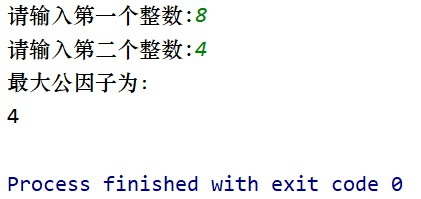
\includegraphics[width=.4\textwidth]{1.1.jpg}\;\;\;\;\;\;\;\;\;\;\;\;\;\;\;\;\;\;\;\;\;\;\;\;
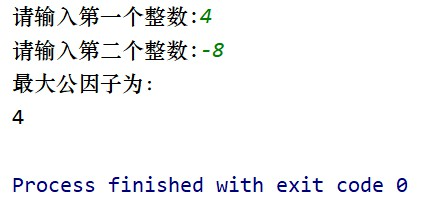
\includegraphics[width=.4\textwidth]{1.2.jpg}\\ \\
\par
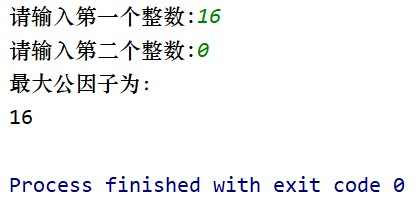
\includegraphics[width=.4\textwidth]{1.3.jpg}\;\;\;\;\;\;\;\;\;\;\;\;\;\;\;\;\;\;\;\;\;\;\;\;
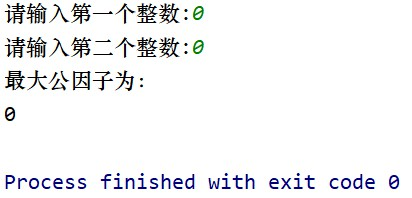
\includegraphics[width=.4\textwidth]{1.4.jpg}

\section{素数}
\subsection{数论基础}
\begin{enumerate}[(1)]
\item \textbf{素数:}一个大于1的正整数$p$,如果仅以1和自身$p$作为其因子,则称p为\textbf{素数}。大于1的非素数的自然数称为\textbf{复合数}
\item \textbf{互素:}如果两个整数$a$和$b$的最大公因子等于1,即$(a,b)=1$,则称$a$和$b$\textbf{互素}。
\end{enumerate}
\subsection{互素的判断}
\par 根据互素的定义,两个整数互素的判断可以通过求它们的最大公因子实现。
\subsubsection{代码实现}
\par 判断两个整数是否互素的函数如下
\begin{python}
  def Relatively_prime(a,b):
    if(a<0):
        a=-a
    if(b<0):
        b=-b
    if(a==0 and b==0):
        gcd=0
    elif(a==0 or b==0):
        gcd=a+b
    else:
        gcd=division_algorithm(a,b)
    if(gcd==1):
        return True
    else: return False
\end{python}
\par 完整程序代码请见附录。
\subsubsection{结果展示}
\par 使用上述程序判断两个整数是否互素的结果如下:\\
\par 
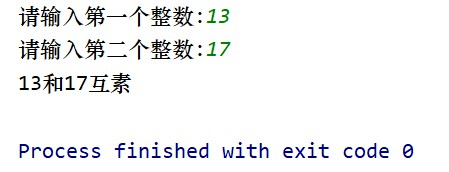
\includegraphics[width=.4\textwidth]{2.1.jpg}\quad\quad\quad\quad\quad\quad
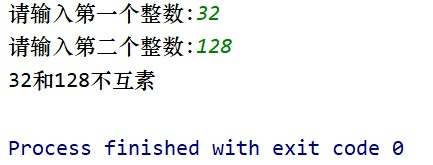
\includegraphics[width=.4\textwidth]{2.2.jpg}

\subsection{Erarosthenes筛法求素数}
\subsubsection{定义}
\par 埃拉托斯特尼筛法是求不超过自然数N(N>1)的所有质数的一种方法。
\par 埃拉托斯特尼是一位古希腊数学家,他在寻找整数N以内的素数时,采用了一种与众不同的方法:先将2一N的各数写在纸上:在2的上面画一个圆圈,然后划去2的其他倍数;
第一个既未画圈又没有被划去的数是3,将它画圈,再划去3的其他倍数;现在既未画圈又没有被划去的第一个数是5,将它画圈,
并划去5的其他倍数……依此类推,一直到所有小于或等于N的各数都画了圈或划去为止。这时,画了圈的以及未划去的那些数正好就是小于N的素数\cite{ref4}。

\subsubsection{代码实现}
\par Erarosthenes筛法寻找素数的代码如下:
\begin{python}
def sieve_func(n):
    prime=[]
    sieve = [True] * (n+1)
    for i in range(2, n):
        if sieve[i]:
            prime.append(i)
            for j in range(i * i, n, i):
                sieve[j] = False
    return prime

n=input("请输入素数的范围n:")
print(sieve_func(int(n)))
\end{python}
\subsubsection{结果展示}
\par 用Erarosthenes筛法寻找1000以内的素数,结果如下:
\par 
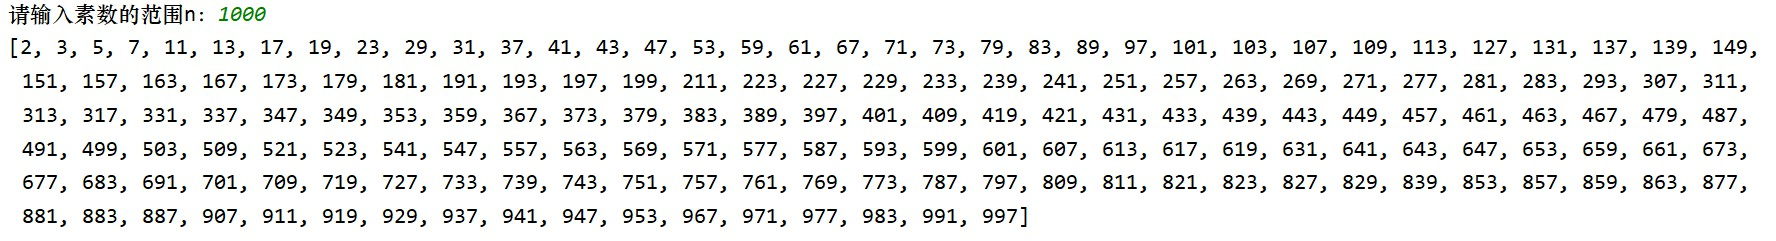
\includegraphics[width=.9\textwidth]{2.3.jpg}
\par 下面我们对程序进行修改,以计算n较大时Erarosthenes筛法的运行速度。
修改后的程序代码请见附录。
\par 分别取$n=100000,n=10000000,n=100000000$,得到结果:
\par
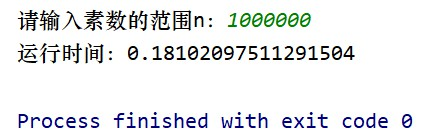
\includegraphics[width=.4\textwidth]{2.4.jpg}
\par
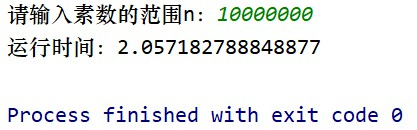
\includegraphics[width=.4\textwidth]{2.5.jpg}
\par
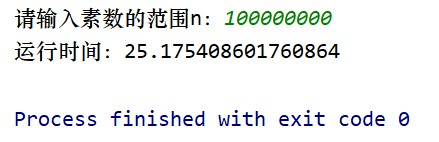
\includegraphics[width=.4\textwidth]{2.6.jpg}
\par 由结果分析可得,使用Erarosthenes筛法寻找100000000以内的素数的速度是比较快的。

\section{同余的应用}
\par 十九世纪初,现代数论第一人的数学家高斯,出版了《算术研究》一
书,并在其中提出了同余的概念及一次同余式组的解法,极大地丰富了数学的内容,为现代同余理论
的发展奠定了牢固的基础.。同余理论在初等数论中占有重要的地位,是研究整数问题的重要手段\cite{ref5}。
\subsection{数论基础}
\begin{enumerate}[(1)]
\item \textbf{同余}:设n为自然数,a,b为任意两个整数,若$a-b$能被$n$除尽,则称$a$与$b$模$n$同余,记为
\[a\equiv  b\quad (mod \quad n)\]
此时,n除a所得的余数与n除b所得的余数相同。
\item \textbf{同余的基本性质}:
  \begin{enumerate}[1)]
  \item 对所有的$a$,$a\equiv a\; (mod\; n)$;
  \item 若$a\equiv b\; (mod\; n)$,则$b\equiv a\; (mod\; n)$
  \item 若$a\equiv b\; (mod\; n)$,$b\equiv c\; (mod\; n)$则$a\equiv c\; (mod\; n)$。
  \end{enumerate}
\item \textbf{解同余方程:}给定整数$a$,正整数$m$,求整数$x$,使\[x\equiv a\; (mod\; m)\]
这称为解同余方程问题。此时$x=a+km$(k为任一整数)是同余方程的所有解。
\item \textbf{扩展欧几里得算法:}是辗转相除法的扩展,已知整数$a,b$,扩展欧几里得算法可以再
求得a,b的最大公因子的同时,找到整数$x,y$,使得:\[ax+by=\operatorname{gcd}(a,b)\]
在本节中,扩展欧几里得算法将用来在中国剩余定理中计算模反元素(也叫模逆元)。
\end{enumerate}
\subsection{同余判断}
\par 判断两个整数是否同余是同余的基本应用。其实现依据于同余的定义。
\subsubsection{代码实现}
\par 判断两个整数是否同余的代码如下:
\begin{python}
def Congruence_judgment(a,b,n):
  if((a-b)%n==0):
      return True
  else:
      return False

a=int(input("请输入第一个整数:"))
b=int(input("请输入第二个整数:"))
n=int(input("请输入模n:"))

if(Congruence_judgment(a,b,n)):
  print("{}与{}模{}同余".format(a,b,n))
else:
  print("{}与{}模{}不同余".format(a,b,n))
\end{python}
\subsubsection{结果展示}
\par 以下展示使用判断同余程序判断两个整数是否模一个整数同余:\\
\par 
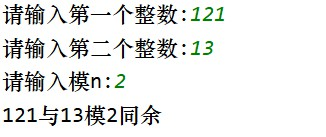
\includegraphics[width=.4\textwidth]{3.1.jpg}\\
\par 
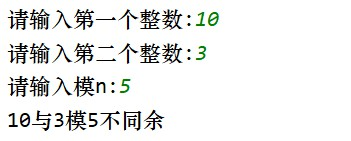
\includegraphics[width=.4\textwidth]{3.2.jpg}
\subsection{中国剩余定理}
\subsubsection{定义}
\par 中国剩余定理也称为孙子定理,是中国古代求解一次同余式组的方法,是数论中一个重要定理,
来源于我国古代的经典数学著作《孙子算经》中的算术题:
“今有物不知其数,三三数之剩二,五五数之剩三,七七数之剩二,问物几何?”
\par 其给出的解法为:“三、三数之剩二,置一百四十;五、五数之剩三,置六十三;七、七数之剩二,置三十,
并之,得二百三十三。以二百一十减之,即得。凡三、三数之剩一,则置七十;五、五数之剩一,则置二十一;
七、七数之剩一,则置十五。一百六以上,一百五减之,即得。”它的算法即为:
\[2 \times 70+3 \times 21+2 \times 15=233,\]再减去105,直至得到23,即为所求结果。
\par 我国古代数学家秦九韶将“孙子问题”的解答进行了推广形成了中国剩余定理,其解法运用了同余的性质。将其抽象为现在的数学问题
,我们可以得到现代的中国剩余定理为:
\par 设$m_1,m_2,...,m_r$是两两互素的自然数,令$m=m_1m_2\dots m_r=m_iM_i$,即$M_i=m_1\dots m_{i-1}m_{i+1}\dots m_r,i=1,2,\dots,r,$
则方程组
\begin{equation}
  \begin{cases}x \equiv b_{1} & \left(\bmod m_{1}\right) \\ x \equiv b_{2} & \left(\bmod m_{2}\right) \\ \cdots & \\ x \equiv b_{r} & \left(\bmod m_{r}\right)\end{cases}
\end{equation}
的解为
\[x \equiv M_{1}^{\prime} M_{1} b_{1}+M_{2}^{\prime} M_{2} b_{2}+\cdots+M_{r}^{\prime} M_{r} b_{r}(\bmod m),\]
其中$M_i'$是整数,使\[M_{i}^{\prime} M_{i} \equiv 1\left(\bmod m_{i}\right), i=1,2, \cdots, r\]
该方程有且仅有一个小于m的非负整数解。
\subsubsection{代码实现}
\par 中国剩余定理的主函数的代码如下:
\begin{python}
def CRT(b_list,m_list):
  M=1
  for mi in m_list:
      M=M*mi
  #计算Mi
  Mi_list=[]
  for mi in m_list:
      Mi_list.append(M//mi)
  #计算Mi的模逆元
  Mi_inverse=[]
  for i in range(len(Mi_list)):
      Mi_inverse.append(get_inversr(Mi_list[i],m_list[i]))
  #计算解x
  x=0
  for i in range(len(b_list)):
      x+=Mi_list[i]*Mi_inverse[i]*b_list[i]
      x%=M
  return x
\end{python}
\par 通过中国剩余定理求同余方程组的解的完整代码请见附录
\subsubsection{结果展示}
\par 使用程序求解同余方程组
\[\begin{cases}x \equiv 2 & (\bmod 3) \\ x \equiv 3 & (\bmod 5) \\ x \equiv 2 & (\bmod 7)\end{cases}\]
的结果:\\
\par
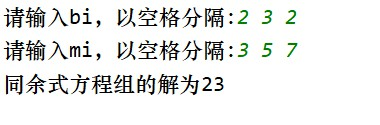
\includegraphics[width=.6\textwidth]{3.3.jpg}
\par 异常输入展示:

\par
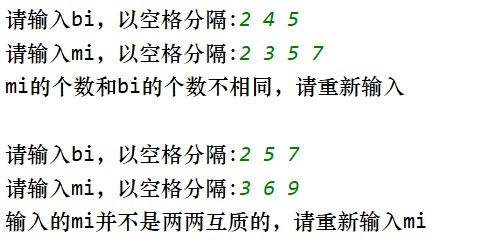
\includegraphics[width=.7\textwidth]{3.4.jpg}



\newpage
\begin{thebibliography}{99}  
  \addcontentsline{toc}{section}{参考文献}
  \bibitem{ref1}牛淑芬,于斐,杨平平,方丽芝.交叉学科背景下信息安全数学基础理论与实践教学方法研究[J].计算机教育,2021(02):149-152.DOI:10.16512/j.cnki.jsjjy.2021.02.035.
  \bibitem{ref2}李瑞琪,高敏芬,贾春福.信息安全数学基础的“讲一练二考三”改革方案设计[J].计算机教育,2016(11):27-30.DOI:10.16512/j.cnki.jsjjy.2016.11.007.
  \bibitem{ref3}裴定一,徐祥,董军武.信息安全数学基础[M].北京:人民邮电出版社,2016
  \bibitem{ref4}杜瑞庆,夏方林.埃拉托斯特尼筛法及改进(C++语言)[J].中国科技信息,2006(18):152-153+156.
  \bibitem{ref5}张双红,高亚楠.论同余理论在生活中的应用[J].吉林省教育学院学报,2017,33(11):181-183.DOI:10.16083/j.cnki.1671-1580.2017.11.053.

  
  \end{thebibliography}
\newpage
\section*{附录}
\addcontentsline{toc}{section}{附录}

\begin{enumerate}[(1)]
\item 辗转相乘法求最大公因子完整代码
\begin{python}
  def division_algorithm(m,n):
      while(n%m!=0):
          m,n=n%m,m
      return m

  a=int(input("请输入第一个整数:"))
  b=int(input("请输入第二个整数:"))
  gcd=0
  if(a<0):
      a=-a
  if(b<0):
      b=-b
  if(a==0 and b==0):
      gcd=0
  elif(a==0 or b==0):
      gcd=a+b
  else:
      gcd=division_algorithm(a,b)
  print("最大公因子为:")
  print(gcd)
\end{python}
\item 整数互素判断完整代码
\begin{python}
def division_algorithm(m,n):
  while(n%m!=0):
      m,n=n%m,m
  return m

def Relatively_prime(a,b):
  if(a<0):
      a=-a
  if(b<0):
      b=-b
  if(a==0 and b==0):
      gcd=0
  elif(a==0 or b==0):
      gcd=a+b
  else:
      gcd=division_algorithm(a,b)
  if(gcd==1):
      return True
  else: return False

a=int(input("请输入第一个整数:"))
b=int(input("请输入第二个整数:"))

if(Relatively_prime(a,b)):
  print("{}和{}互素".format(a,b))
else: 
  print("{}和{}不互素".format(a,b))

\end{python}
\item Erarosthenes筛法寻找素数运行时间计算代码
\begin{python}
  from time import *
  def sieve_func(n):
      prime=[]
      sieve = [True] * (n+1)
      for i in range(2, n):
          if sieve[i]:
              prime.append(i)
              for j in range(i * i, n, i):
                  sieve[j] = False
      return prime
  
  n=input("请输入素数的范围n:")
  begin_time=time()
  sieve_func(int(n))
  end_time=time()
  run_time=end_time-begin_time
  print('运行时间:{}'.format(run_time))
\end{python}
\item 中国剩余定理求解同余方程组完整代码
\begin{python}
#扩展欧几里得算法的函数
def ext_euclid(a, b):     
    if b == 0:         
        return 1, 0, a     
    else:         
        x, y, q = ext_euclid(b, a % b)         
        x, y = y, (x - (a // b) * y)         
        return x, y, q

#运用扩展欧几里得算法求模逆元
def get_inversr(a,b):
    return ext_euclid(a,b)[0]

#中国剩余定理
def CRT(b_list,m_list):
    M=1
    for mi in m_list:
        M=M*mi
    #计算Mi
    Mi_list=[]
    for mi in m_list:
        Mi_list.append(M//mi)
    #计算Mi的模逆元
    Mi_inverse=[]
    for i in range(len(Mi_list)):
        Mi_inverse.append(get_inversr(Mi_list[i],m_list[i]))
    #计算解x
    x=0
    for i in range(len(b_list)):
        x+=Mi_list[i]*Mi_inverse[i]*b_list[i]
        x%=M
    return x

#判断列表中元素是否两两互素
def ifcoprime(ls):
  for i in range(len(ls)):
    for j in range(i+1,len(ls)):
      if ext_euclid(ls[i],ls[j])[2]!=1:
        return 0  


#输入bi,mi
while True:
    m_list=[]
    b_list=[]
    
    b_i=input("请输入bi,以空格分隔:")
    b_i=b_i.split( )
    for i in b_i:
      b_list.append(int(i))
    
    m_i=input("请输入mi,以空格分隔:")
    m_i=m_i.split( )
    for i in m_i:
      m_list.append(int(i))
    
    if len(m_list)!=len(b_list):
      print("mi的个数和bi的个数不相同,请重新输入\n")
    elif ifcoprime(m_list)==0:
      print("输入的mi并不是两两互质的,请重新输入mi\n")
    else:
      break

x=CRT(b_list,m_list)
print("同余式方程组的解为{}".format(x))
\end{python}
\end{enumerate}
\end{document}